\documentclass{article}

\usepackage{hyperref}
\usepackage{pgfplots}
\usepgfplotslibrary{fillbetween}
\pgfplotsset{compat=1.13}

\title{Basics of Economics}
\author{Alvin Lin}
\date{Principles of Microeconomics: August 2016 - December 2016}

\begin{document}

\maketitle

\section{Utility and Demand}
What determines the choices made by a consumer? Where do individual's demand
curves come from? Consumption Possibilities are determined by prices and
income.

\subsection{The Budget Line}
The \textbf{budget line} is the boundary between combinations that an
individual can afford and those that the individual cannot afford. The budget
line is determined by income and prices.

\subsubsection{Preferences and Utility}
Preferences describe an individual's likes and dislikes and how they rank
various bundles of goods. \textbf{Total Utility} is the total benefit or
satisfaction that a person gets from consuming goods. \textbf{Marginal
Utility} is the change in total utility that results from a one unit
increase in the quantity of a good consumed. The Consumer's Problem is to
choose the most preferred bundle among those she can afford, or, to choose
the bundle that gives her the highest utility among those she can afford.
An indifference curve describes all the consumption bundles among which
a consumer is indifferent.

\subsubsection{The Consumer's Problem}
Given some transitive relationship \( X>Y \), \( X<Y \), or \( X\sim Y \),
there exists a function \( u(x,y) \) which yields the total utility of the
goods. The problem is reduced to maximizing \( u(x,y) \). The consumer
chooses a bundle that maximizes utility within the constraints. \par
We will assume positive marginal utility, which means that more is always
better. We will also assume diminishing marginal utility, which means the
increase in utility is smaller the greater the quantity of the good. The
goal is to find the preferred bundle on the budget line.
\begin{center}
  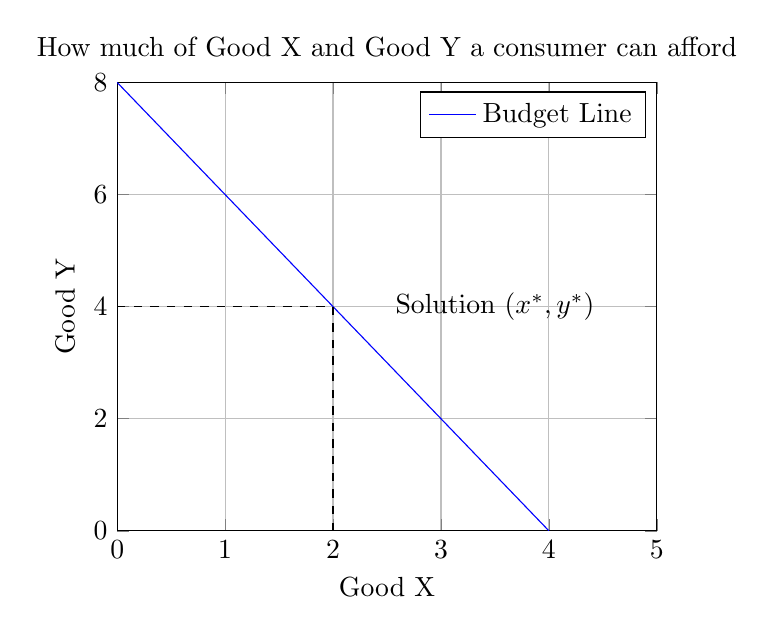
\begin{tikzpicture}
    \begin{axis} [
      title={How much of Good X and Good Y a consumer can afford},
      xlabel={Good X}, ylabel={Good Y},
      xmin=0, xmax=5, ymin=0, ymax=8,
      grid=both
    ]
      \addplot[name path=supply, color=blue] coordinates { (0,8) (4,0) };
      \addlegendentry{Budget Line};
      \addplot[dashed, color=black] coordinates { (2,0) (2,4) };
      \addplot[dashed, color=black] coordinates { (0,4) (2,4) };
      \node[draw=none] at (3.5,4) {Solution \( (x^{*},y^{*}) \)};
    \end{axis}
  \end{tikzpicture}
\end{center}
\[ p_{x}x^{*}+p_{y}y^{*} = m \]
\[ u(x,y) = u_{x}(x)+u_{y}(y) \]
\[ \frac{mu_{x}(x^{*},y^{*})}{p_{x}} = \frac{mu_{y}(x^{*},y^{*})}{p_{y}} \]

\subsubsection{Example}
\[ m = 40 \quad p_{x} = 8 \quad p_{y} = 4 \]
\begin{center}
  \begin{tabular}{|c|c|c|c|}
    \hline
    \( x \) & \( u_{x} \) & \(y \) & \( u_{y} \) \\ \hline
    0       & 0           & 0      & 0           \\ \hline
    1       & 50          & 1      & 25          \\ \hline
    2       & 90          & 2      & 123         \\ \hline
    3       & 122         & 3      & 159         \\ \hline
    4       & 150         & 4      & 183         \\ \hline
    5       & 176         & 5      & 205         \\ \hline
    6       & 200         & 6      & 225         \\ \hline
    7       & 222         & 7      & 238         \\ \hline
    8       & 242         & 8      & 243         \\ \hline
    9       & 259         & 9      & 255         \\ \hline
    10      & 295         & 10     & 260         \\ \hline
  \end{tabular}
\end{center}
Find (x,y) on the budget line, and find the bundle on the budget line that
gives the highest utility:
\begin{center}
  \begin{tabular}{|c|c|c|c|c|}
    \hline
    \( x \) & \( y \) & \( u_{x} \) & \( u_{y} \) & \( u(x,y) \) \\ \hline
    0       & 10      & 0           & 260         & 260          \\ \hline
    1       & 8       & 50          & 248         & 298          \\ \hline
    2       & 6       & 90          & 225         & 315          \\ \hline
    3       & 4       & 122         & 183         & 305          \\ \hline
    4       & 2       & 150         & 123         & 273          \\ \hline
    5       & 0       & 176         & 0           & 176          \\ \hline
  \end{tabular}
\end{center}
\( u(x,y) \) is maximized at (2,6).

\begin{center}
  You can find all my notes at \url{http://omgimanerd.tech/notes}. If you have
  any questions, comments, or concerns, please contact me at
  alvin@omgimanerd.tech
\end{center}

\end{document}
